%%%%%%%%%%%%%%%%%%%%%%%%%%%%%%%%%%%%%%%%%%%%%%%%%%%%%%%%%%
%%%%%%%%%%%%%%%%%%%%%%%%%%%%%%%%%%%%%%%%%%%%%%%%%%%%%%%%%%
\chapter[RepulsionPak: Deformation-Driven Element Packing \newline with Repulsion Forces]
{RepulsionPak: Deformation-Driven Element Packing with Repulsion Forces}
%%%%%%%%%%%%%%%%%%%%%%%%%%%%%%%%%%%%%%%%%%%%%%%%%%%%%%%%%%
%%%%%%%%%%%%%%%%%%%%%%%%%%%%%%%%%%%%%%%%%%%%%%%%%%%%%%%%%%



%%%%%%%%%%%%%%%%%%%%%%%%%%%%%%%%%%%%%%%%%%%%%%%%%%%%%%%%%%
%%%%%%%%%%%%%%%%%%%%%%%%%%%%%%%%%%%%%%%%%%%%%%%%%%%%%%%%%%
\section{Introduction}
%%%%%%%%%%%%%%%%%%%%%%%%%%%%%%%%%%%%%%%%%%%%%%%%%%%%%%%%%%
%%%%%%%%%%%%%%%%%%%%%%%%%%%%%%%%%%%%%%%%%%%%%%%%%%%%%%%%%%



%%%%%%%%%%%%%%%%%%%%%%%%%%%%%%%%%%%%%%%%%%%%%%%%%%%%%%%%%%
%%%%%%%%%%%%%%%%%%%%%%%%%%%%%%%%%%%%%%%%%%%%%%%%%%%%%%%%%%
\section{Previous Work}
%%%%%%%%%%%%%%%%%%%%%%%%%%%%%%%%%%%%%%%%%%%%%%%%%%%%%%%%%%
%%%%%%%%%%%%%%%%%%%%%%%%%%%%%%%%%%%%%%%%%%%%%%%%%%%%%%%%%%


%%%%%%%%%%%%%%%%%%%%%%%%%%%%%%%%%%%%%%%%%%%%%%%%%%%%%%%%%%
%%%%%%%%%%%%%%%%%%%%%%%%%%%%%%%%%%%%%%%%%%%%%%%%%%%%%%%%%%
\section{System Overview}
%%%%%%%%%%%%%%%%%%%%%%%%%%%%%%%%%%%%%%%%%%%%%%%%%%%%%%%%%%
%%%%%%%%%%%%%%%%%%%%%%%%%%%%%%%%%%%%%%%%%%%%%%%%%%%%%%%%%%




\begin{figure}[h]
\centering
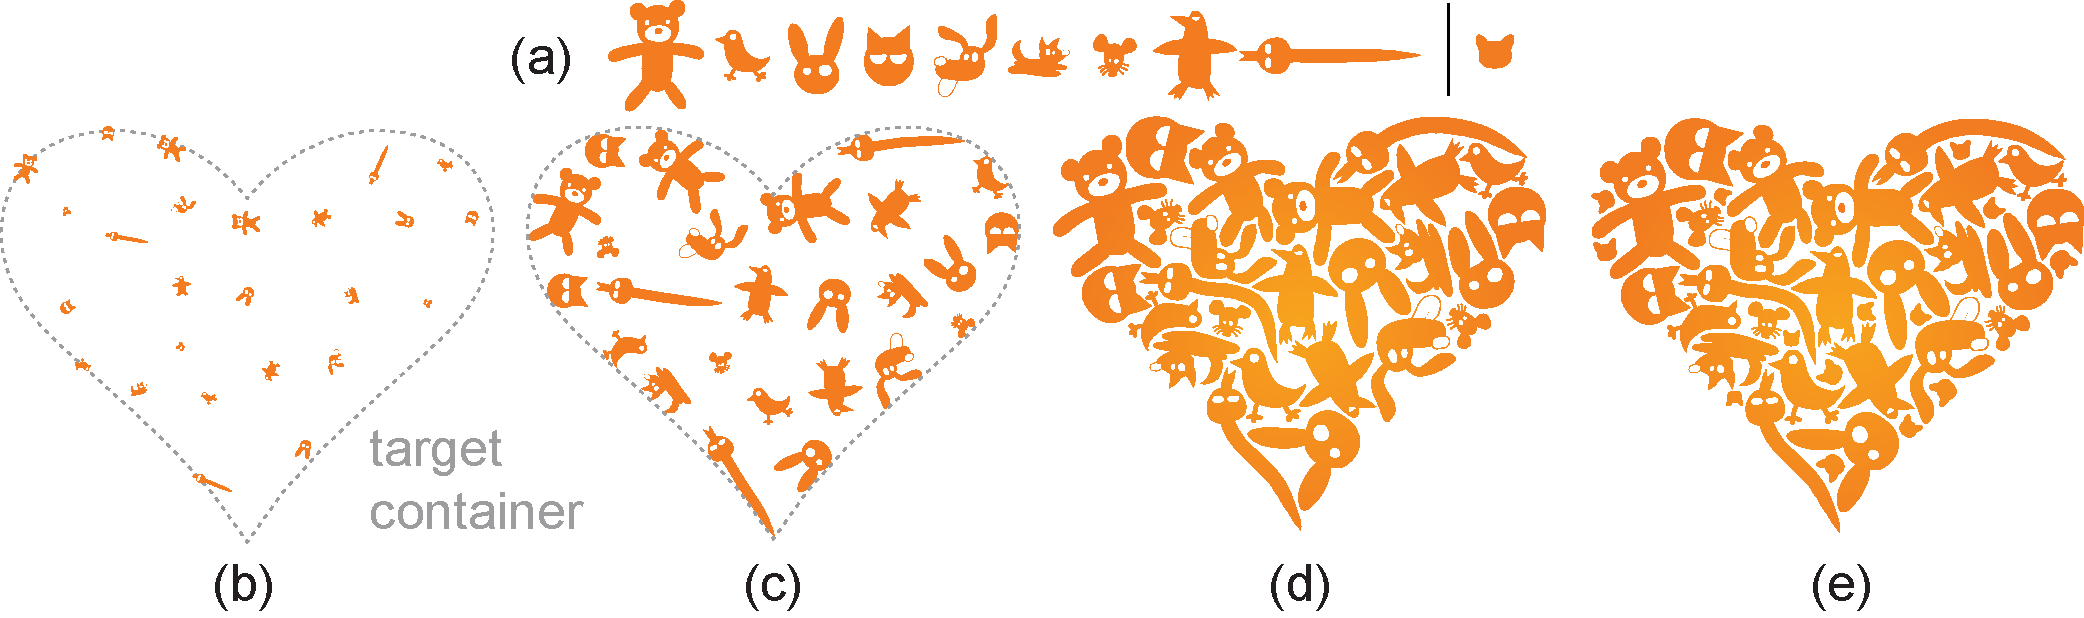
\includegraphics[width=1.0\textwidth]{figures/repulsionpak/pipeline.pdf} 
\caption[RepulsionPak pipeline]
{\label{fig_repulsionpak_pipeline} 
RepulsionPak pipeline. }
\end{figure}

\begin{figure}[h]
\centering

\includegraphics[width=5cm]{figures/repulsionpak/pipeline_defviz_csk.pdf}
\caption[Element deformation]{
	\label{fig_defviz}
	Some of the elements in the final packing in Fig.~\ref{fig_repulsionpak_pipeline}, 
	showing the effect of deformation in our simulation.
}
\end{figure}


%%%%%%%%%%%%%%%%%%%%%%%%%%%%%%%%%%%%%%%%%%%%%%%%%%%%%%%%%%
%%%%%%%%%%%%%%%%%%%%%%%%%%%%%%%%%%%%%%%%%%%%%%%%%%%%%%%%%%
\section{Preprocessing}
%%%%%%%%%%%%%%%%%%%%%%%%%%%%%%%%%%%%%%%%%%%%%%%%%%%%%%%%%%
%%%%%%%%%%%%%%%%%%%%%%%%%%%%%%%%%%%%%%%%%%%%%%%%%%%%%%%%%%

\begin{figure}[t] %%% ELEMENT IMAGE
\centering
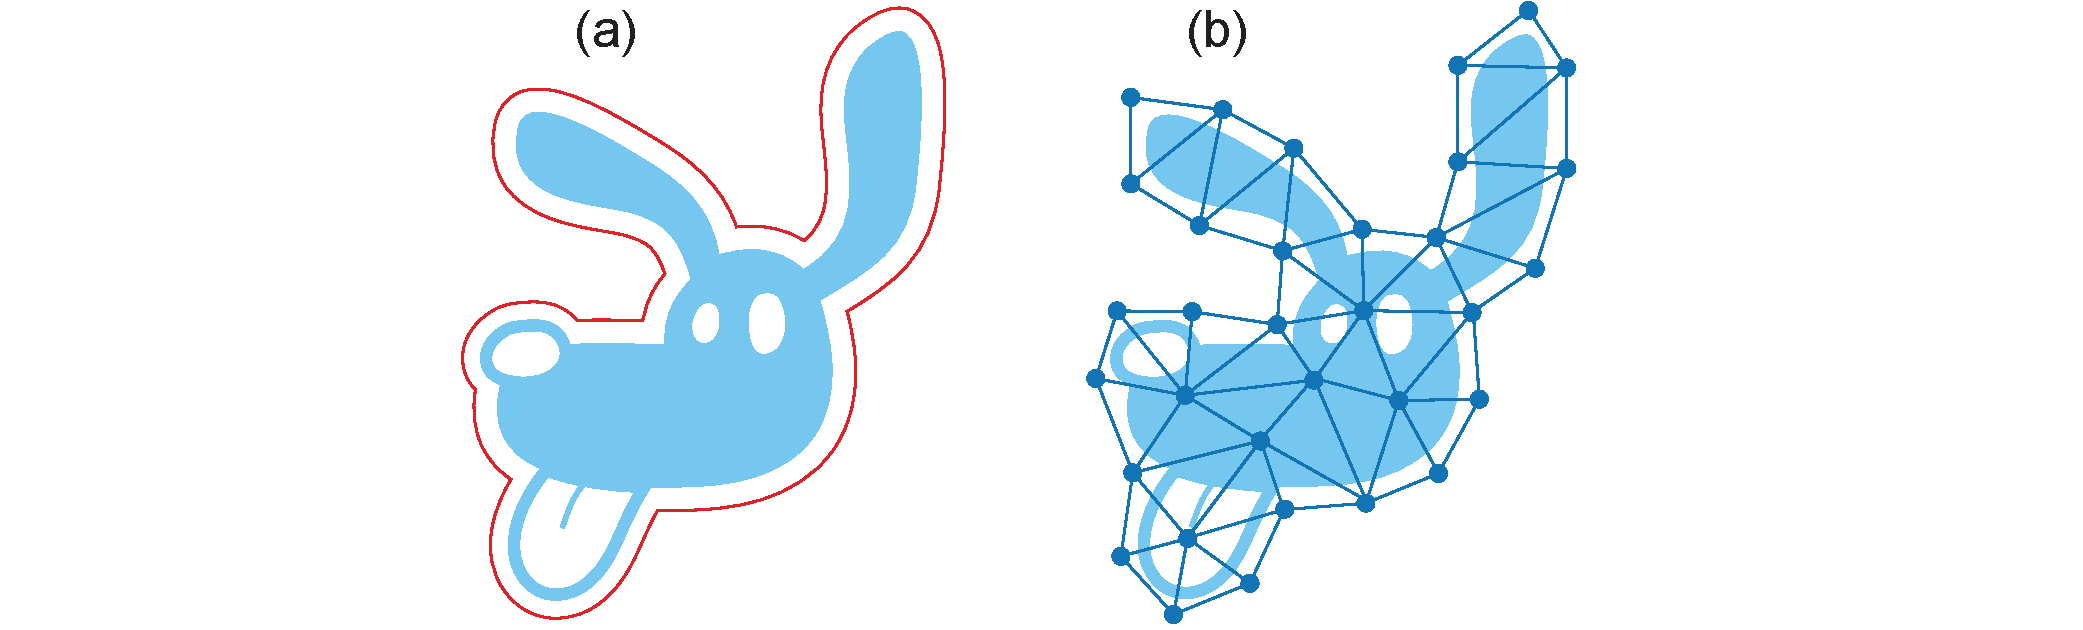
\includegraphics[width=4.5cm]{figures/repulsionpak/element_skin_triangles_2.pdf}
\caption[Element discretization]{
	\label{fig_elements_image}
	\newtext{An illustration of element discretization for preprocessing.}
	(a) An element with its boundary displaced to create a skin, drawn in red.
	(b) A triangle mesh with boundary vertices on the skin.
}
\end{figure}

\begin{figure*}[t]
\centering
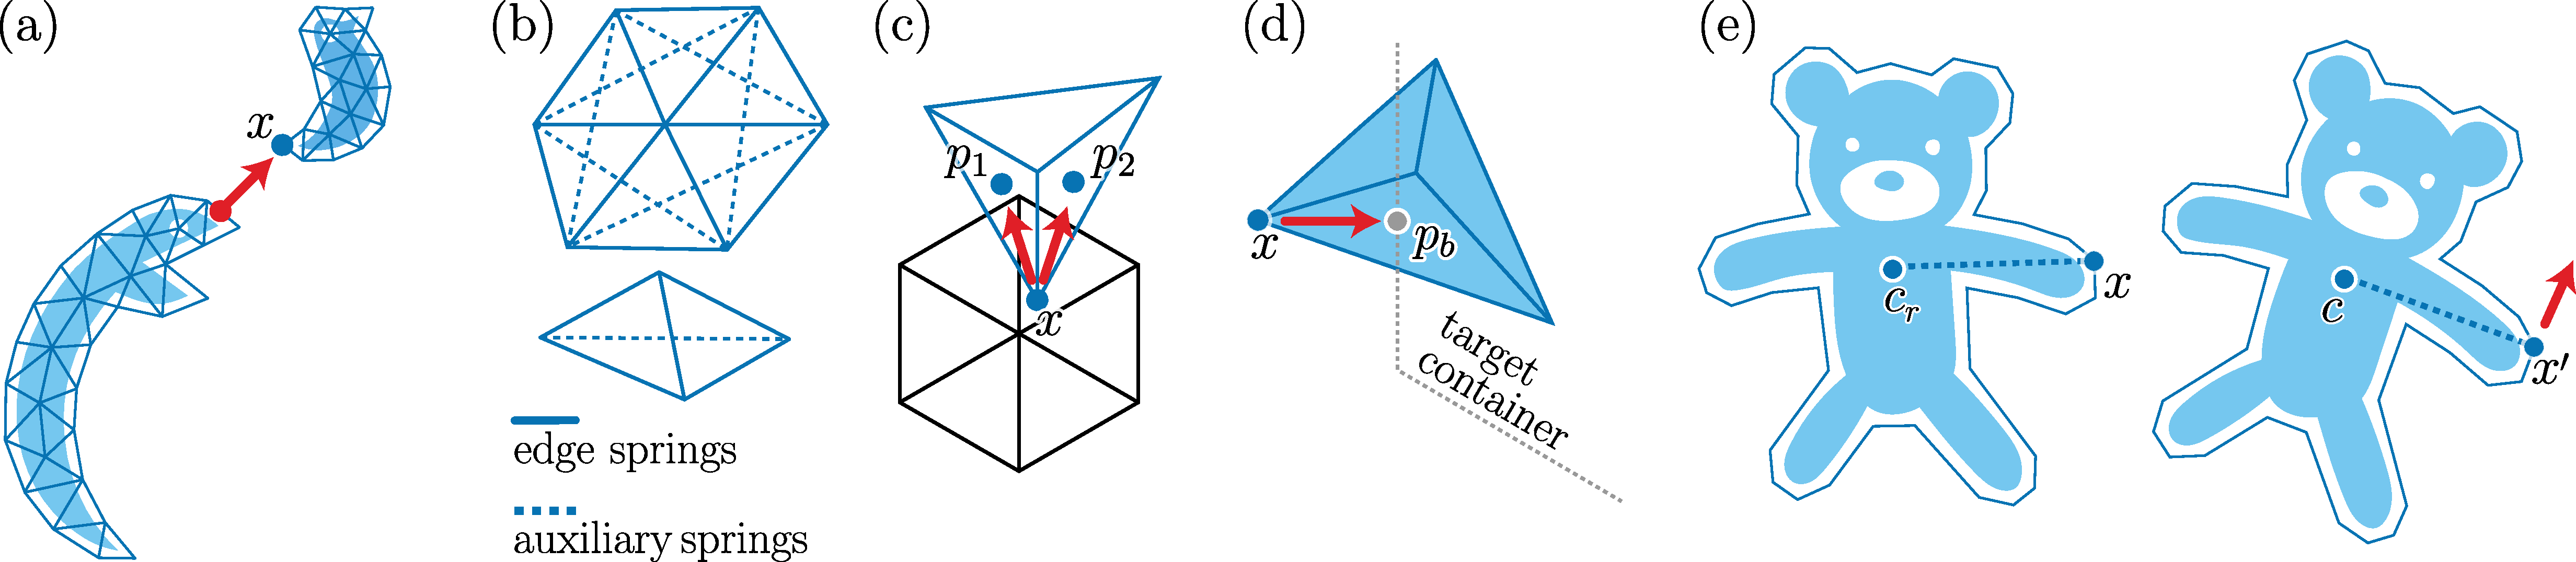
\includegraphics[width=1.0\textwidth]{figures/repulsionpak/all_forces.pdf}
\caption[Forces]{
\label{fig_forces}
Illustrations of the forces in our simulation.
\;\textbf{(a)~Repulsion force}:
The closest point on the snake's mesh
repels a vertex $\bm{x}$ in the bird mesh.
\textbf{(b)~Edge force}: 
We generate edge forces using
edge springs and auxiliary springs.
\textbf{(c)~Overlap force}: 
Centres of triangles $\bm{p_1}$ and $\bm{p_2}$ attract a vertex
$\bm{x}$ that lies in the interior of another mesh.
\;\textbf{(d)~Boundary force}: A vertex $\bm{x}$ moves toward $\bm{p_b}$,
the closest point on a target container, when it is outside the container.
\textbf{(e)~Torsional force}: We restrict the orientation of the element by generating 
a torsional force at every boundary vertex $\bm{x}$
to restore its angular position relative to $\bm{c}$, 
the center of mass of the element.
\mynote
{
xs should be bold.
Should include negative space edges.
}
}
\end{figure*}



%%%%%%%%%%%%%%%%%%%%%%%%%%%%%%%%%%%%%%%%%%%%%%%%%%%%%%%%%%
%%%%%%%%%%%%%%%%%%%%%%%%%%%%%%%%%%%%%%%%%%%%%%%%%%%%%%%%%%
\section{Simulation}
%%%%%%%%%%%%%%%%%%%%%%%%%%%%%%%%%%%%%%%%%%%%%%%%%%%%%%%%%%
%%%%%%%%%%%%%%%%%%%%%%%%%%%%%%%%%%%%%%%%%%%%%%%%%%%%%%%%%%


%%%%%%%%%%%%%%%%%%%%%%%%%%%%%%%%%%%%%%%%%%%%%%%%%%%%%%%%%%
%%%%%%%%%%%%%%%%%%%%%%%%%%%%%%%%%%%%%%%%%%%%%%%%%%%%%%%%%%
\subsection{Element Growth}
%%%%%%%%%%%%%%%%%%%%%%%%%%%%%%%%%%%%%%%%%%%%%%%%%%%%%%%%%%
%%%%%%%%%%%%%%%%%%%%%%%%%%%%%%%%%%%%%%%%%%%%%%%%%%%%%%%%%%




%%%%%%%%%%%%%%%%%%%%%%%%%%%%%%%%%%%%%%%%%%%%%%%%%%%%%%%%%%
%%%%%%%%%%%%%%%%%%%%%%%%%%%%%%%%%%%%%%%%%%%%%%%%%%%%%%%%%%
\subsection{Stopping Criteria}
%%%%%%%%%%%%%%%%%%%%%%%%%%%%%%%%%%%%%%%%%%%%%%%%%%%%%%%%%%
%%%%%%%%%%%%%%%%%%%%%%%%%%%%%%%%%%%%%%%%%%%%%%%%%%%%%%%%%%



%%%%%%%%%%%%%%%%%%%%%%%%%%%%%%%%%%%%%%%%%%%%%%%%%%%%%%%%%%
%%%%%%%%%%%%%%%%%%%%%%%%%%%%%%%%%%%%%%%%%%%%%%%%%%%%%%%%%%
\section{Shape Matching}
\label{shape_matching}
%%%%%%%%%%%%%%%%%%%%%%%%%%%%%%%%%%%%%%%%%%%%%%%%%%%%%%%%%%
%%%%%%%%%%%%%%%%%%%%%%%%%%%%%%%%%%%%%%%%%%%%%%%%%%%%%%%%%%



\begin{figure}[t]
\centering

\includegraphics[width=0.3\columnwidth]{figures/repulsionpak/descriptor_2.pdf}
\caption[A local shape descriptor for shape matching]
{\label{fig_shape_matching}
\newtext{An illustration of a local shape descriptor with $n = 3$. 
These segments have varying arclengths but they all have the same value
of $\tau$, the integral of absolute curvature along their lengths.}
}
\end{figure}
\begin{figure}
\centering
\includegraphics[width=0.95\columnwidth]{figures/repulsionpak/rhino_shape_matching_bitmap.pdf} 
\caption[A demonstration of shape matching of leaf shapes inside a rhinoceros]
{\label{rhino_packing}
{ 
A demonstration of shape matching of leaf shapes inside a rhinoceros. 
(a) We detect nine salient features, namely sharp convex corners, and 
assign an element to each.
(b) A spring holds each element in place.
(c) The final result.
}
}
\end{figure}

%%%%%%%%%%%%%%%%%%%%%%%%%%%%%%%%%%%%%%%%%%%%%%%%%%%%%%%%%%
%%%%%%%%%%%%%%%%%%%%%%%%%%%%%%%%%%%%%%%%%%%%%%%%%%%%%%%%%%
\section{Results}
%%%%%%%%%%%%%%%%%%%%%%%%%%%%%%%%%%%%%%%%%%%%%%%%%%%%%%%%%%
%%%%%%%%%%%%%%%%%%%%%%%%%%%%%%%%%%%%%%%%%%%%%%%%%%%%%%%%%%

\begin{figure*}
  \centering
  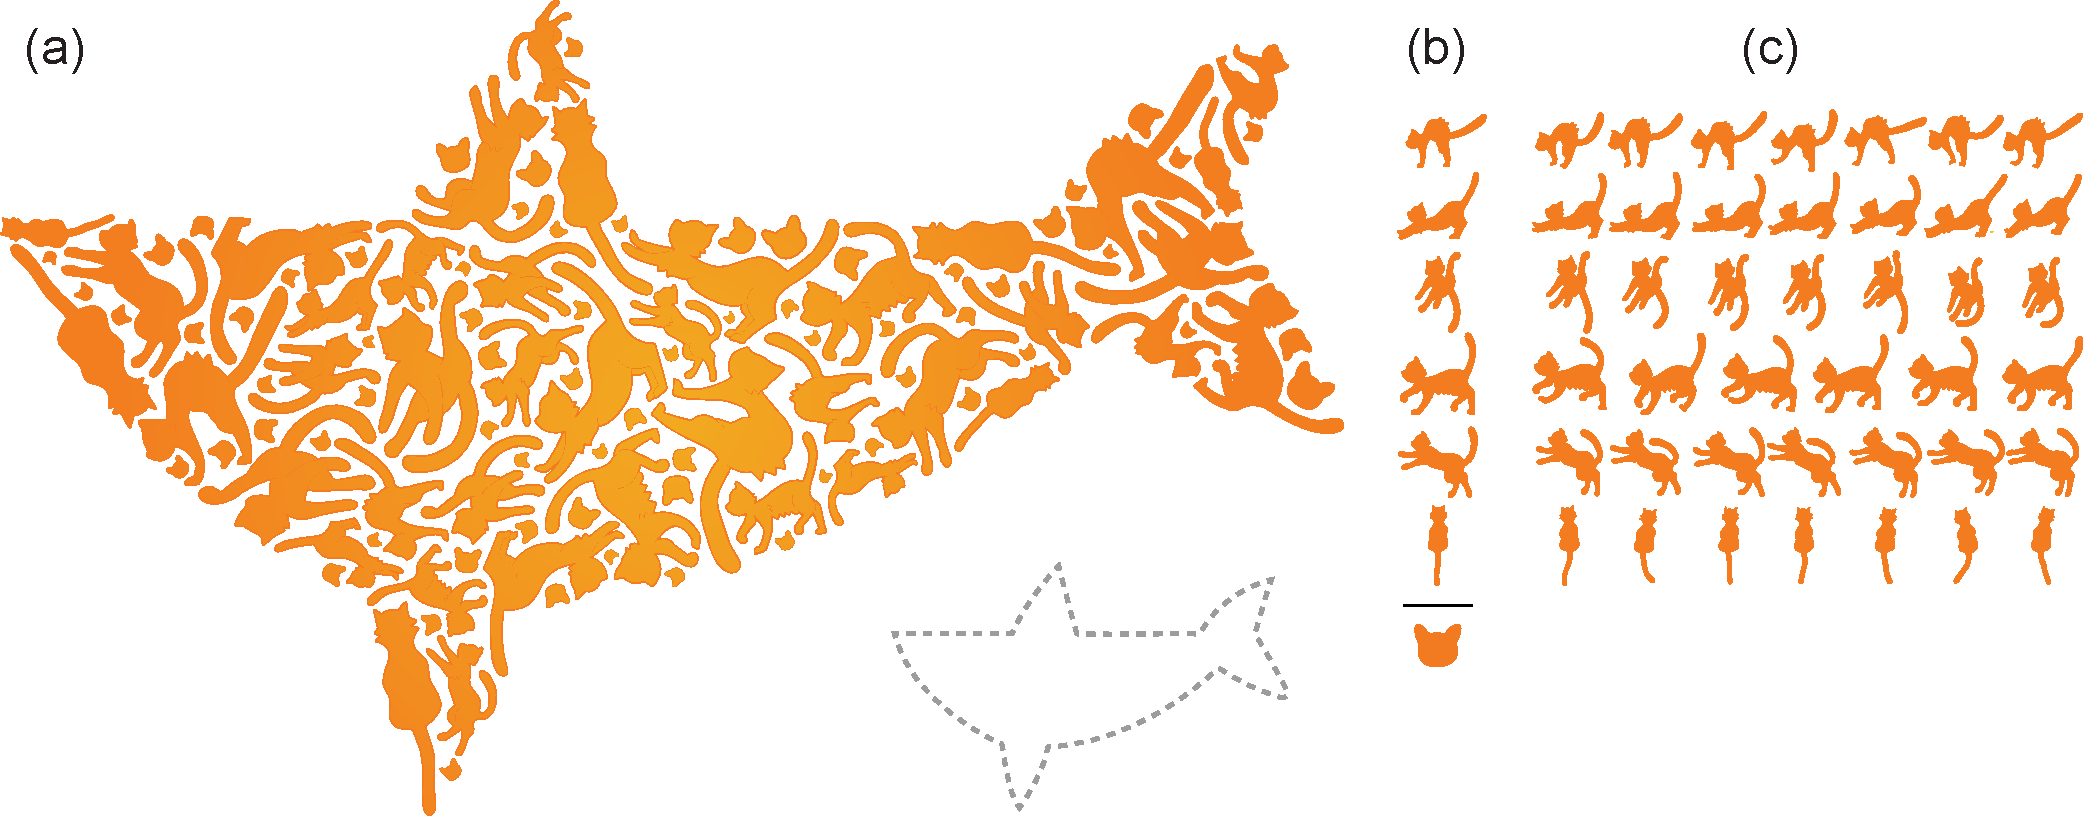
\includegraphics[width=1.0\textwidth]{figures/repulsionpak/cat_whale_04}
  \caption[A packing of a cat]
  {
  \label{cat_packing}
           A packing of six cat elements inside a fish-shaped target container. 
           Controllable deformation and repulsion forces allow the elements to deform,
           efficiently filling the container and creating a uniform distribution of
           negative space. We then reduce the remaining negative space by placing smaller
           cat heads. The gradient fill was added as a post-process.}
\end{figure*}

\begin{figure*}
\centering
\includegraphics[width=1.0\textwidth]{figures/repulsionpak/allresults.pdf} 
\caption[Three packings created using RepulsionPak: Birds, Bats, and Butterflies]
{\label{three_packings} Three packings created using RepulsionPak: \newline Birds, Bats, and Butterflies. The results are visually appealing overall,
though some birds' tails suffer from excessive deformation in
the packing on the left.}
\end{figure*}

\begin{figure*}
\centering
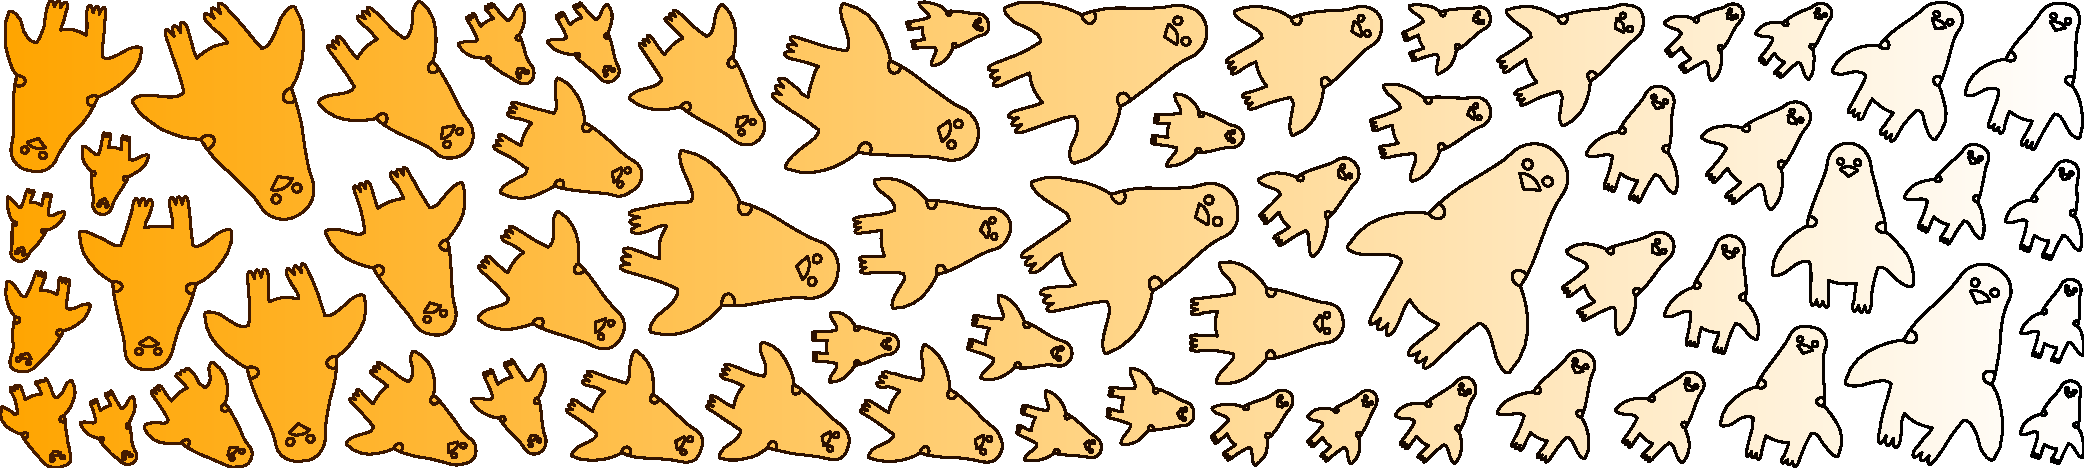
\includegraphics[width=1.0\textwidth]{figures/repulsionpak/giraffe_penguin.pdf}
\caption[A packing that demonstrates torsional forces]
{\label{giraffe_penguin_packing}
A packing that demonstrates torsional forces.
The packing uses copies of a single element shape, but every copy is given a rest orientation between $0^\circ$
and $180^\circ$, based on its horizontal position in the container.  In the final packing the elements transition
from upright to upside-down, recreating an illusion in which giraffe heads become penguins.}
\end{figure*}

%\begin{minipage}{\textwidth}
\begin{figure}
\centering
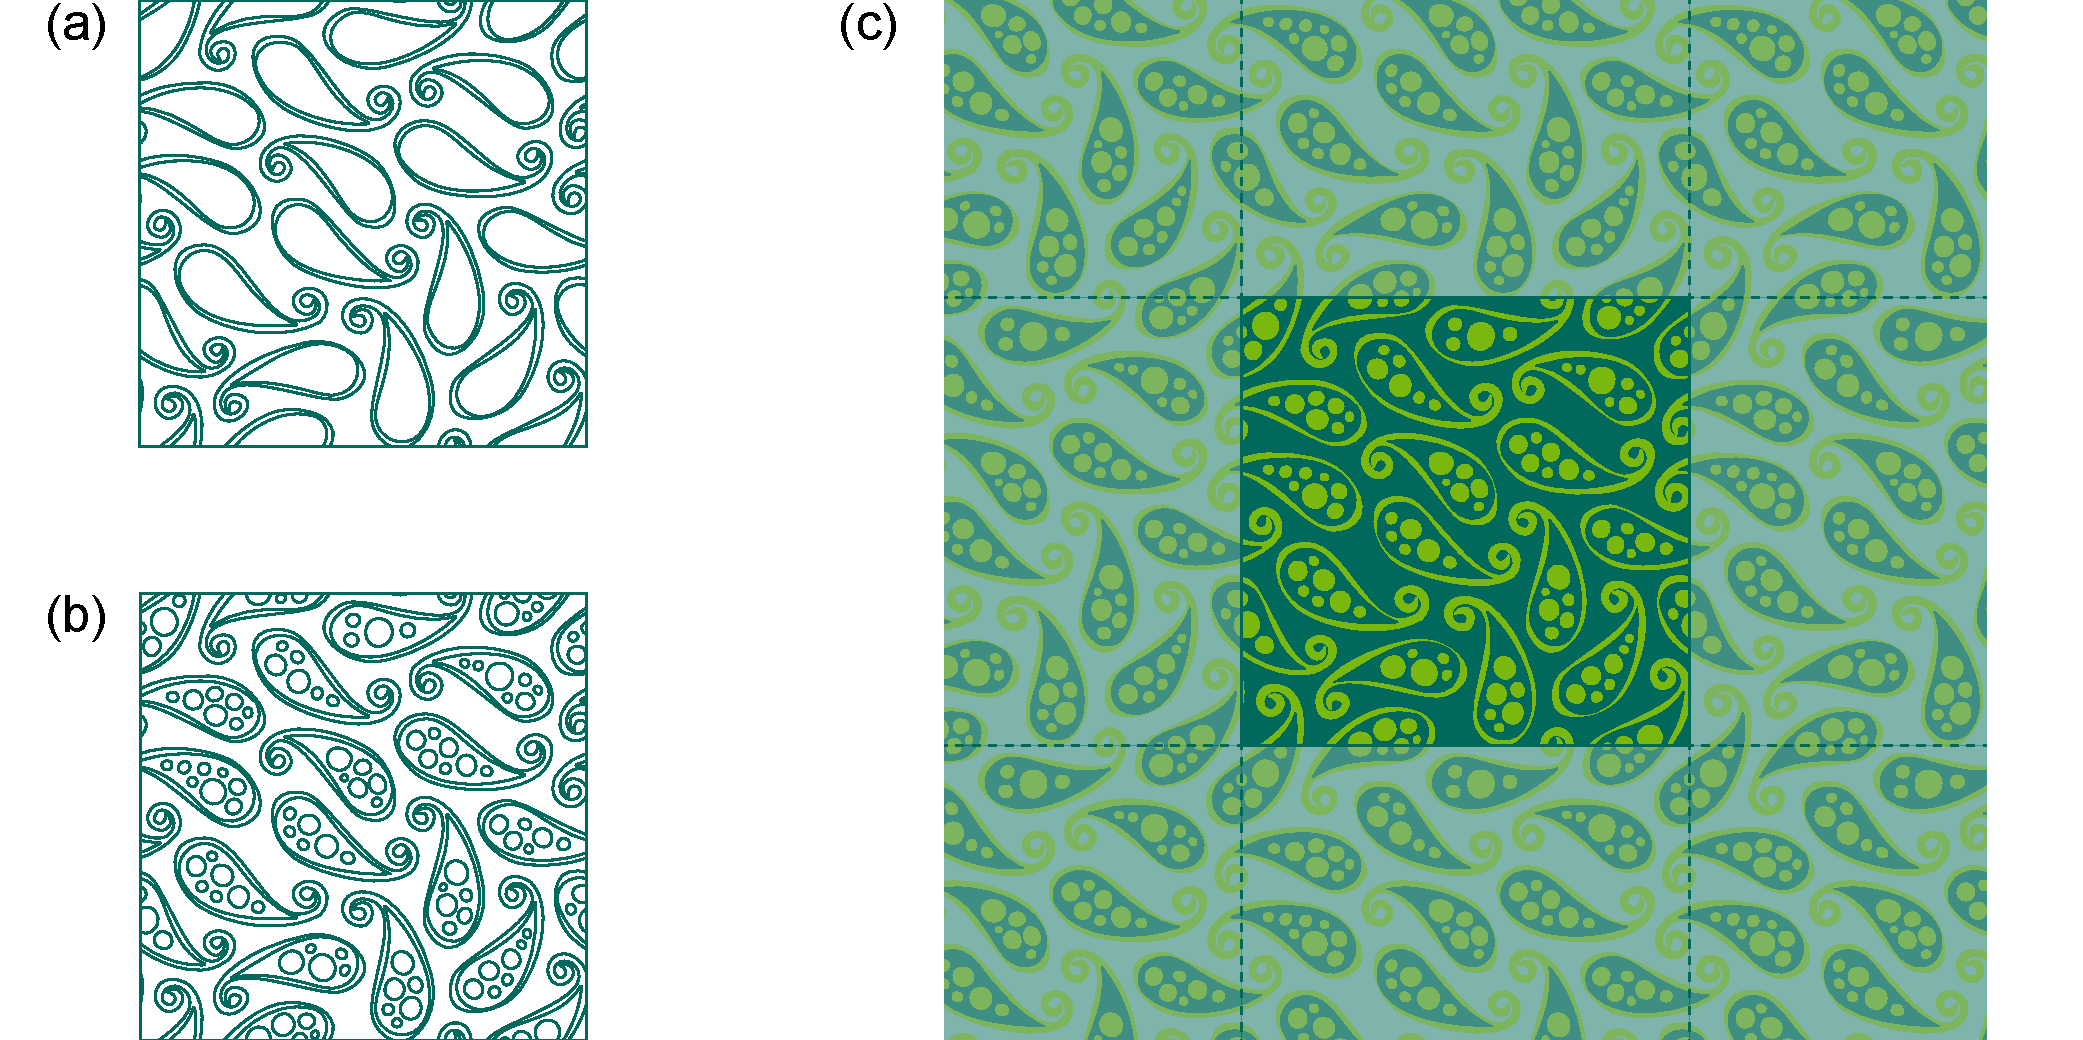
\includegraphics[width=0.95\columnwidth]{figures/repulsionpak/paisley_new.pdf} 
\vspace{-10pt}
\caption[A paisley-inspired toroidal packing that can tile the plane]
{\label{paisley_packing}
A paisley-inspired toroidal packing that can tile the plane. 
           (a) An initial paisley packing.
           (b) In a separate simulation, we fill each paisley with circles to demonstrate a packing inside a packing.
           (c) The final result.
}
\end{figure}

\begin{figure}
\centering

\includegraphics[width=0.85\columnwidth]{figures/repulsionpak/bad_results.pdf} 
\vspace{-12pt}
\caption[Two demonstrations of how extreme parameter values can lead to \newline 
	low-quality results]
	{\label{bad_results}
Two demonstrations of how extreme parameter values can lead to
	low-quality results.  In~(a), we allow repulsion to overwhelm element
	shape by setting $k_r$ to 200 and $k_e$ to 20; the resulting packing 
	has even negative space, but elements suffer from high deformation
	and self intersections.  In~(b), we minimize repulsion and prioritize
	orientation by setting $k_e$, $k_t$, and $k_r$ to 200, 100, and 50,
	respectively.  The elements deviate minimally from their original shapes 
	and orientations, but cannot fill the container effectively.
}
\end{figure}


%%%%%%%%%%%%%%%%%%%%%%%%%%%%%%%%%%%%%%%%%%%%%%%%%%%%%%%%%%
%%%%%%%%%%%%%%%%%%%%%%%%%%%%%%%%%%%%%%%%%%%%%%%%%%%%%%%%%%
\section{Conclusions}
%%%%%%%%%%%%%%%%%%%%%%%%%%%%%%%%%%%%%%%%%%%%%%%%%%%%%%%%%%
%%%%%%%%%%%%%%%%%%%%%%%%%%%%%%%%%%%%%%%%%%%%%%%%%%%%%%%%%%